\section{Projet}
\subsection{Les livrables}
\begin{frame}
    \frametitle{\color{white}Les livrables}
    \begin{block}{Trois livrables demandés}
      \begin{itemize}
         \item Une étude détaillée d'OpenPGP et de GnuPG.
         \item Une interface graphique permettant de faciliter la compréhension et l'utilisation de GnuPG.
         \item Une étude des limites, et une implantation d'une attaque sur les identifiants de clefs PGP.
       \end{itemize} 
    \end{block}
\end{frame}

\subsection{L'attaque}
\begin{frame}
  \frametitle{\color{white}Attaque}
  \begin{block}{Lexique}
    \begin{itemize}
      \item Clef PGP = clef de certification encapsulée dans un paquet PGP
      \item L'empreinte est le résultat de la fonction de hachage sha-1 sur la clef
      \item L'identifiant d'une clef est la troncature des 8 derniers caractères d'une empreinte. Le nom de l'utilisateur ne suffit pas à identifier une clef, car il n'est pas unique.
    \end{itemize}
    \end{block}
  \begin{block}{Attaque sur les identifiants de clef}
    \begin{itemize}
      \item L'objectif de cette attaque est de forger une clef pour tromper un utilisateur important une clef depuis un serveur.
      %\item Documentation sur les limites de GnuPG.
    \end{itemize}
  \end{block}
\end{frame}

\begin{frame}
  \frametitle{\color{white}Attaque}
  \begin{block}{ }
  Cette attaque est issue du dépôt github de Micah Lee (trollwot), elle-même issue du code source du projet Monkeysphere.
  \end{block}
  \begin{block}{Fonctionnement de l'attaque}
      \begin{itemize}
        \item Crée une clef RSA.
        \item Modifie la date de création jusqu'à ce que le haché soit identique à la clef voulue.
        \item Fabrique un paquet PGP avec la clef RSA pour qu'il soit importable dans GnuPG.
        \item Le temps est de maximum 4 jours avec les ordinateurs de la faculté qui calculent 12 000 hachés par seconde.
      \end{itemize}
  \end{block}
\end{frame}

\begin{frame}
  \frametitle{\color{white}Les contraintes de l'attaque}
  \begin{block}{Date de création}
      \begin{itemize}
        \item La date de création doit être supérieure à 1970 l'année 0 pour les machines.
        \item La date de création doit être inférieure à la date d'aujourd'hui.
      \end{itemize}
    \end{block}
    \medbreak
    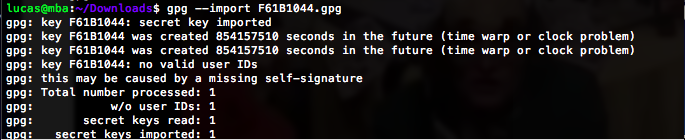
\includegraphics[scale=0.42]{attaque.png}
\end{frame}

\subsection{L'interface graphique}
\begin{frame}
    \frametitle{\color{white}GuiPG}
    \begin{block}{Fonctionnalités}
      \begin{itemize}
        \item Gestion d'un trousseau de clefs gpg.
        \item Opérations cryptographiques.
        \item Représentation de la toile de confiance.
        \item Visualisation des commandes nécessaires pour chaque action.
      \end{itemize}
    \end{block}
\end{frame}

\begin{frame}
  \frametitle{\color{white}GuiPG}
  \begin{block}{Gestion d'un trousseau de clefs gpg}
      \begin{itemize}
        \item Création de clefs / sous clefs.
        \item Suppression de clef principale.
        \item Certification de clef.
        \item Modification de la confiance.
        \item Ajouter un identifiant utilisateur.
        \item Importation / Exportation de clefs depuis un fichier.
      \end{itemize}
    \end{block}
    \pause
    \begin{block}{Opérations cryptographiques}
      \begin{itemize}
        \item Chiffrer un fichier
	  \begin{itemize}
	   \item Possibilité de choisir plusieurs destinataires à la fois.
	   \item Possibilité d'anonymiser les destinataires.
	  \end{itemize}
        \item Déchiffrer un fichier.
        \item Vérifier la signature d'un fichier.
      \end{itemize}
    \end{block}
\end{frame}


\section{Les risques survenus}
  \subsection{Risques organisationnels}
    \begin{frame}
      \frametitle{\color{white}Risques organisationnels}
      \begin{block}{Incompatibilité d'emploi du temps}
	\begin{itemize}
	  \item Deux membres sont passés en Master GIL.
	  \item Difficultés pour se réunir et travailler ensemble.
	\end{itemize}
      \end{block}
      \begin{block}{Perte d'effectif - Risque R\_09}
      	\begin{itemize}
      	  \item Deux membres ont quitté le projet durant le premier sprint.
      	  \item Sous-effectif pour les travaux prévus.
      	\end{itemize}
      \end{block}
    \end{frame}
    
    \begin{frame}
      \frametitle{\color{white}Risques organisationnels}
      \begin{alertblock}{Impacts}
      	\begin{itemize}
      	 \item Tâches non finalisées à temps.
      	 \item Accumulation de retard.
      	 \item 2 semaines de retard sur la première livraison.
      	 \item 1ère livraison non validée.
      	\end{itemize}
      \end{alertblock}
      \pause
      \begin{exampleblock}{Plan d'action}
        \begin{itemize}
          \item Réunion pour évaluer l'état d'avancement du projet.
          \item Proposition à la cliente d'une redéfinition du périmètre du projet.
          \item Négociation et priorisation des tâches et des délais / Sprints avec la cliente.
        \end{itemize}
      \end{exampleblock}
    \end{frame}

  \subsection{Risques techniques}
    \begin{frame}
      \frametitle{\color{white}Maîtrise des outils}
      \begin{block}{Maîtrise des outils - Risque R\_01}
        Certains des membres n'étaient pas assez formés sur les outils utilisés\\
        (git, Qt, C++, gpg)
      \end{block}
      \pause
      \begin{alertblock}{Impact}
        \begin{itemize}
          \item Perte de temps sur les tâches prévues
        \end{itemize}
      \end{alertblock}
      \pause
      \begin{exampleblock}{Solutions}
        \begin{itemize}
          \item Réunion d'installation et de formation aux outils 
        \end{itemize}
      \end{exampleblock}
    \end{frame}

    \begin{frame}
      \frametitle{\color{white}Fonctionnement technique de GnuPG}
      \begin{block}{Communication avec le processus GnuPG}
        \begin{itemize}
	         \item Impossibilité de récupérer certains retours des commandes -> Impossibilité de traitement.
          \item GnuPG utilise directement un tty comme entrée / sortie pour certaines commandes.
        \end{itemize}
      \end{block}
      \pause
      \begin{alertblock}{Impacts}
        \begin{itemize}
          \item Impossibilité d'avancer dans l'implantation des commandes prévues.
        \end{itemize}
      \end{alertblock}
      \pause
      \begin{exampleblock}{Solutions}
        \begin{itemize}
          \item Inspection du code source de GnuPG et de son comportement
          \item Utilisation de bibliothèques prévues pour manipuler GnuPG - {\color{red}Proscrit}
	    \begin{itemize}
	     \item Perte de la visualisation des commandes gpg => Exigence indispensable EF\_16
	    \end{itemize}
          \item Réalisation d'un pseudo-terminal via l'api système POSIX - {\color{green}Adopté}
	    \begin{itemize}
	     \item impose un système UNIX => perte de compatibilité Windows (Exigence optionnelle E0\_12)
	    \end{itemize}
        \end{itemize}
      \end{exampleblock}
    \end{frame}

\section{Bilan du projet}
  
  \subsection{Résultats du projet}
  \begin{frame}
    \frametitle{\color{white}Vue globale du projet}
  \begin{tabular}{|l|l|l|}
    \hline
    \multicolumn{1}{|c|}{\cellcolor{gray} \color{white}Catégories} & \multicolumn{1}{|c|}{\cellcolor{gray} \color{white}Livraison} & \multicolumn{1}{|c|}{\cellcolor{gray} \color{white}Livraison initiale} \\
    \hline
    \cellcolor{white}\color{green}Fondation & \multicolumn{1}{|c|}{\cellcolor{white}\color{black}1} & \multicolumn{1}{|c|}{\cellcolor{white}\color{black}1} \\
    \hline
    \cellcolor{white}\color{green}Mécanisme multi-instance & \multicolumn{1}{|c|}{\cellcolor{white}\color{black}1} & \multicolumn{1}{|c|}{\cellcolor{white}\color{black}1} \\    
    \hline
    \cellcolor{white}\color{green}Gestion des profils & \multicolumn{1}{|c|}{\cellcolor{white}\color{black}1} & \multicolumn{1}{|c|}{\cellcolor{white}\color{black}1} \\
    \hline
    \cellcolor{white}\color{blue}Gestion des clefs & \multicolumn{1}{|c|}{\cellcolor{white}\color{black}2} & \multicolumn{1}{|c|}{\cellcolor{white}\color{black}1} \\
    \hline
    \cellcolor{white}\color{green}Vue des commandes et retours GPG & \multicolumn{1}{|c|}{\cellcolor{white}\color{black}2} & \multicolumn{1}{|c|}{\cellcolor{white}\color{black}1} \\
    \hline
    \cellcolor{white}\color{blue}Opérations cryptographiques & \multicolumn{1}{|c|}{\cellcolor{white}\color{black}2} & \multicolumn{1}{|c|}{\cellcolor{white}\color{black}2} \\
    \hline
    \cellcolor{white}\color{blue}\'{E}diteur & \multicolumn{1}{|c|}{\cellcolor{white}\color{black}2} & \multicolumn{1}{|c|}{\cellcolor{white}\color{black}2} \\
    \hline
    \cellcolor{white}\color{red}Attaque & \multicolumn{1}{|c|}{\cellcolor{white}\color{black}2} & \multicolumn{1}{|c|}{\cellcolor{white}\color{black}3} \\
    \hline
    \cellcolor{white}\color{red}\'{E}tude gestion des clefs & \multicolumn{1}{|c|}{\cellcolor{white}\color{black}} & \multicolumn{1}{|c|}{\cellcolor{white}\color{black}1} \\
    \hline
    \cellcolor{white}\color{red}\'{E}tude des opérations cryptographiques & \multicolumn{1}{|c|}{\cellcolor{white}\color{black}} & \multicolumn{1}{|c|}{\cellcolor{white}\color{black}2} \\
    \hline
    \cellcolor{white}\color{red}\'{E}tude gestion de la toile de confiance & \multicolumn{1}{|c|}{\cellcolor{white}\color{black}} & \multicolumn{1}{|c|}{\cellcolor{white}\color{black}2} \\
    \hline
    \cellcolor{white}\color{red}\'{E}tude des limites & \multicolumn{1}{|c|}{\cellcolor{white}\color{black}} & \multicolumn{1}{|c|}{\cellcolor{white}\color{black}3} \\
    \hline
    \cellcolor{white}\color{red}Toile de confiance statique (graphe) & \multicolumn{1}{|c|}{\cellcolor{white}\color{black}} & \multicolumn{1}{|c|}{\cellcolor{white}\color{black}2} \\
    \hline
    \cellcolor{white}\color{red}Toile dynamique (graphe) & \multicolumn{1}{|c|}{\cellcolor{white}\color{black}} & \multicolumn{1}{|c|}{\cellcolor{white}\color{black}3} \\
    \hline
  \end{tabular}
\end{frame}

\subsection{Améliorations et rétrospective}
  \begin{frame}
    \frametitle{\color{white}Ce qu'on pourrait améliorer}
    \begin{block}{Axes d'améliorations}
      Améliorations de l'interface GuiPG :
      \begin{itemize}
        \item Affiner la gestion de clef.
        \item Ajouter une visualisation sous forme de graphe de la toile de confiance.
        \item Développer l'éditeur de texte.
        \item Personnaliser l'interface.
      \end{itemize}
      Améliorations de l'attaque :
      \begin{itemize}
        \item Paralléliser le calcul des hashs de la clef sur CPU.
        \item Implanter l'attaque sur carte graphique (OpenCL, CUDA).
      \end{itemize}
    \end{block}
    
  \end{frame}

  \begin{frame}
  \frametitle{\color{white}Si c'était à refaire}
    \begin{block}{Rétrospective}
    Approfondir l'étude de faisabilité lors de la phase d'avant projet.
      \begin{itemize}
        \item Expérimenter plus en détail le logiciel GnuPG en ligne de commande.
        \item S'assurer de la compréhension et de la maîtrise des outils de la part de chacun.
        \item Utiliser Python.
      \end{itemize}
    \end{block}


  \end{frame}
